\documentclass{article}

\usepackage[preprint]{neurips_2025}
\usepackage{amsmath,amssymb,amsthm}
\usepackage{graphicx}
\usepackage{subcaption}
\usepackage{booktabs}
\usepackage{multirow}
\usepackage{hyperref}
\usepackage{microtype}
\usepackage{xcolor}
\usepackage{pgfplots}
\pgfplotsset{compat=1.18}
\usepgfplotslibrary{groupplots}
\usepackage{tcolorbox}
\tcbuselibrary{listings}
% \usepackage{listings}
\lstset{
  language=Python,
  basicstyle=\ttfamily\scriptsize,
  keywordstyle=\bfseries,
  commentstyle=\color{gray},
  stringstyle=\color{gray},
  breaklines=true,
  frame=single,
  numbers=left,
  numberstyle=\tiny\color{gray},
  xleftmargin=1.5em,
  framexleftmargin=1.5em,
}

% Theorem environments
\newtheorem{proposition}{Proposition}
\newtheorem{corollary}{Corollary}
\newtheorem{remark}{Remark}
\theoremstyle{definition}
\newtheorem{definition}{Definition}

% Notation
\newcommand{\bx}{\boldsymbol{x}}
\newcommand{\bc}{\boldsymbol{c}}
\newcommand{\ba}{\boldsymbol{a}}
\newcommand{\bD}{\boldsymbol{D}}
\newcommand{\bC}{\boldsymbol{C}}
\newcommand{\calR}{\mathcal{R}}
\newcommand{\EE}{\mathbb{E}}
\newcommand{\RR}{\mathbb{R}}
\newcommand{\TODO}[1]{\textcolor{red}{[TODO: #1]}}

\definecolor{proxyblue}{HTML}{1f78b4}

\title{ACE: An Analytical Rate Proxy for Compression-aware Optimization}

\author{%
  \TODO{authors}
}

\begin{document}
\maketitle

\begin{abstract}
    Gradient-based optimization over image codecs is hindered by the non-differentiability of quantization and entropy coding, and existing differentiable rate proxies require training a codec-specific surrogate network. 
    We introduce ACE (AC-Entropy proxy), an analytical, training-free, differentiable estimator of block-transform codec bitrate derived directly from the codec's own transform-coding pipeline. 
    We show theoretically that ACE converges to the true differential entropy of the AC coefficients, that the DCT is a near-optimal transform for natural images under a standard Markov-1 model, and that ACE's gradient aligns with the gradient of the true block-transform codec rate—together, these justify its use as an optimization signal. 
    Empirically, we confirm that ACE closely tracks the measured HEVC bitrate across quality levels. 
    We demonstrate ACE's versatility across four applications spanning pixel space, perturbation space, feature space, and generative sampling: purifying adversarial examples without knowledge of the attack or model, augmenting training data to improve corruption robustness, constructing perturbations that better survive lossy compression, regularizing intermediate features for bandwidth-efficient split inference, and guiding diffusion sampling toward more compressible outputs. 
    In each setting, ACE requires no auxiliary training and adds no learned parameters, making it a lightweight, drop-in tool for any pipeline that needs a differentiable notion of coded image rate.
\end{abstract}

\begin{center}
    Code: \url{https://github.com/ThomasWalker1/ACE}
\end{center}

\begin{figure}[ht]
    \centering
    \begin{subfigure}[b]{0.24\textwidth}
        \centering
        \caption*{\small Original}
        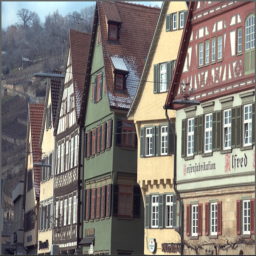
\includegraphics[width=\textwidth]{figures/original.png}
    \end{subfigure}
    \begin{subfigure}[b]{0.24\textwidth}
        \centering
        \caption*{\small ACE Heatmap}
        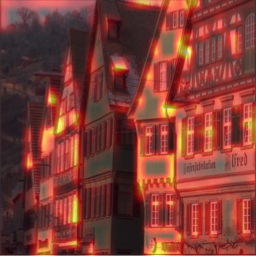
\includegraphics[width=\textwidth]{figures/dct_heatmap.png}
    \end{subfigure}
    \begin{subfigure}[b]{0.24\textwidth}
        \centering
        \caption*{\small PGD Noise}
        
\includegraphics[width=\textwidth]{figures/pgd_noise.png}
    \end{subfigure}
    \begin{subfigure}[b]{0.24\textwidth}
        \centering
        \caption*{\small Purification Residual}
        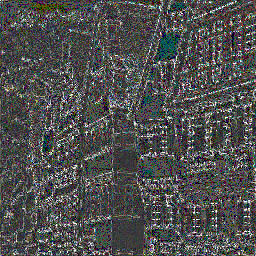
\includegraphics[width=\textwidth]{figures/purification_residual.png}
    \end{subfigure}
    \caption{%
        \textbf{ACE provides an informative compression-aware gradient signal.}
        We propose an analytical, training-free, differentiable proxy for block-transform codec bitrate (ACE) and demonstrate its utility for gradient-based, compression-aware optimization in pixel space, among other applications.
        The ACE heatmap (second panel) provides per-block AC coefficient energy overlaid on the original image.
        When applied to adversarial perturbations constructed with PGD (third panel), ACE can purify the noise (fourth panel) and restore classifier performance. 
        When applied to clean images during training, the same proxy gradient steps can augment training data to improve the robustness of image classifiers.
    }
    \label{fig:main}
\end{figure}

% ---------------------------------------------------------------------------
\section{Introduction}
% ---------------------------------------------------------------------------

Gradient-based optimization in image codecs is hindered by quantization and entropy coding, both of which are non-differentiable.
The standard workaround is a differentiable rate proxy---a smooth function whose gradient with respect to pixel values points in the same direction as the true codec rate~\citep{balle2018variational,guo2026generative}.

Every existing proxy requires training.
\citet{balle2018variational} uses additive uniform noise and a learned entropy model; \citet{mentzer2018conditional} a per-pixel conditional distribution; \citet{guo2026generative} a diff-BPG network that simulates BPG's full intra prediction and entropy coding pipeline.
All three undergo a second training stage specific to a given codec configuration, which requires codec-labeled data.

We observe that block-transform codecs' rate---HEVC being the common standard for video/image compression---is dominated by the entropy of AC DCT-II coefficients~\citep{sullivan2012hevc}, and that those coefficients can be computed \emph{analytically} from any image in closed form.
ACE works by relaxing the subsequent encoding of the coefficients in the block-transform codec pipeline using a Gaussian soft assignment, yielding a fully differentiable, parameter-free rate estimator.
Thus, ACE's gradient is well-defined everywhere, and we show that it points in the direction of decreasing AC coefficient entropy---precisely the direction that lowers a block-transform codec's coded bitrate (\S\ref{sec:proxy}).

Differentiable rate proxies serve as an efficient tool for problems in which a signal must be steered toward compressibility.
We demonstrate that ACE is as a lightweight, parameter-free, drop-in tool for four such tasks across perturbation space (\S\ref{sec:adv_pur} and \S\ref{sec:survival}), pixel space (\S\ref{sec:aug}), feature space (\S\ref{sec:split}), and generative sampling (\S\ref{sec:diffguide}).

% ---------------------------------------------------------------------------
\section{Background}
\label{sec:background}
% ---------------------------------------------------------------------------

Block-transform codecs are the family of video/image compression standards that underlie most modern lossy compression, with HEVC (High Efficiency Video Coding, also known as H.265) as the leading example~\citep{sullivan2012hevc}. 
Like JPEG before it, a block-transform codec compresses an image by splitting it into $B\times B$ blocks, transforming each block from pixel values into a frequency representation, and then entropy-coding that representation.

The transform used is the DCT-II (the two-dimensional discrete cosine transform), which converts a block of pixel intensities into a set of coefficients describing how much energy the block contains at each spatial frequency. 
The single lowest-frequency coefficient, the DC term, captures the block's average intensity and is coded separately via intra prediction; the remaining 63 coefficients, the AC coefficients, capture the block's edges and texture at increasingly fine spatial scales.
Because natural image blocks are smooth almost everywhere, most AC coefficients are close to zero, and it is precisely this concentration --- the fact that the AC coefficient distribution has low entropy --- that the entropy coder (CABAC, in HEVC) exploits to produce a small file. 
Conversely, a block with textured, noisy, or adversarially perturbed content spreads energy across many AC coefficients, raising their entropy and inflating the coded bitrate. 
This is why a block-transform codec's coded rate is dominated by the entropy of the AC coefficients~\citep{sullivan2012hevc}.

To obtain differentiable proxies of this procedure: \citet{balle2018variational} replace quantization with additive uniform noise and a learned entropy model for end-to-end learned compression.
\citet{mentzer2018conditional} uses a per-pixel conditional distribution.
\citet{guo2026generative} trains a diff-BPG network that simulates BPG's full pipeline, then uses it to fine-tune a diffusion preprocessor.
All learned surrogates require codec-labeled training data and are specific to a given codec or QP range.

Closed-form, training-free rate estimation has existed in the form of Lagrangian rate-distortion optimization (RDO) to facilitate mode-decision inside HEVC/H.264 encoders, precisely because running the actual entropy coder at every candidate mode is too slow~\citep{sullivan1998rdo}. 
These estimates are derived from the same DCT/entropy-coding pipeline that ACE models, but they are used to rank a discrete set of candidate encoder modes, not to take a gradient step on the input itself.

ACE's contribution is therefore not that it is analytical---RDO cost estimates are too---but that it is differentiable with respect to the image or feature map itself, letting gradient steps be taken directly in pixel, feature, or latent space toward arbitrary downstream objectives (\S\ref{sec:applications}), rather than only ranking a finite set of encoder-internal choices.

After establishing theoretically that ACE is an accurate and reliable differentiable rate proxy (\S \ref{sec:proxy}), we explore its utility in various machine learning applications, such as robustness.
Robustness requires that the outputs of machine learning models remain stable under small input perturbations.
However, gradient-based attacks (FGSM~\citep{goodfellow2014explaining}, PGD~\citep{madry2017towards}) can produce perturbations that, while small in $\ell_\infty$ norm, fool machine learning systems.
JPEG compression~\citep{guo2018countering} purifies adversarial examples via hard DCT quantization; our proxy is a soft, differentiable analog.

% ---------------------------------------------------------------------------
\section{ACE: An Analytical and Differentiable Rate Proxy}
\label{sec:proxy}
% ---------------------------------------------------------------------------

We first define ACE and show that it empirically tracks HEVC bitrate, then provide theoretical guarantees explaining why it does so and why its gradients are reliable.
The definition is closed-form and requires no training data.
The theory establishes three properties---entropy consistency, near-optimality under the standard natural-image model, and gradient alignment with the true block-transform codec rate---that together justify the use of its gradient as an optimization signal.

\subsection{Definition and Calibration}
\label{sec:definition}

\begin{definition}[ACE]
\label{def:proxy}
Let $\bx \in [0,1]^{H \times W \times C}$ be an image.
Partition $\bx$ into non-overlapping $B \times B$ blocks.
For each block: subtract the block mean; apply the orthonormal 2D DCT-II to obtain $\bC = \bD\tilde{b}\bD^\top$; collect the AC coefficients $\ba = \left(\bC_{ij}\right)_{(i,j)\neq(0,0)}$.
Let $\bc = (c_1,\ldots,c_M)$ be equally-spaced centers on $[-l,\,l]$ and set $\sigma>0$.
The soft-histogram probability for bin $m$ is set as
\begin{equation*}
  \hat{p}_m = \frac{1}{|\ba|}\sum_{a \in \ba}
    \frac{\exp(-\tfrac{(a-c_m)^2}{2\sigma^2})}
         {\sum_{m'}\exp(-\tfrac{(a-c_{m'})^2}{2\sigma^2})},
\end{equation*}
such that the ACE rate of $\bx$ is $\hat{r}(\bx) = -\sum_{m} \hat{p}_m \log_2 \hat{p}_m$.
\end{definition}

ACE replicates a block-transform codec's intra coding pipeline in a closed, differentiable form: block mean subtraction approximates DC intra prediction (HEVC mode 1); orthonormal DCT-II is equivalent to the codec's transform; AC soft-histogram entropy approximates the CABAC output.
No quantization simulation is included; ACE estimates the entropy of unquantized AC coefficients, which correlates strongly with the quantized coded rate (Table~\ref{tab:calibration}).

ACE is applied independently to each color channel of $\bx$ and the per-channel values are summed to form $\hat{r}(\bx)$.
HEVC codes chroma at reduced resolution with separate QP offsets.
For simplicity, the calibration in Table~\ref{tab:calibration} compares the summed RGB proxy against HEVC's total reported bitrate (luma + chroma combined).
The high within-CRF correlations ($r\ge0.90$) confirm that this simplified color treatment does not impair the gradient signal.

Definition~\ref{def:proxy} requires the specification of different constants; we set $B=8$, $M=64$, $l=1.5$, and $\sigma=3.0/M$.
AC coefficients outside the range $[-l,l]$ are soft-assigned to the nearest boundary bin by the Gaussian kernel.
Empirically, only $0.017\%$ of Kodak~\citep{kodak1993} AC coefficients and $0.030\%$of a 500-image ImageNet~\citep{deng2009imagenet} sample fall outside $[-1.5, 1.5]$, confirming that the range covers the effective support of natural-image distributions.

We validate ACE against the measured HEVC bitrate on all 24 Kodak images at CRF $\in\{22,27,32,37,42,47\}$ (144 (image, CRF) pairs).
ACE is constant per image (QP-agnostic by design), so the 144-pair correlation has two orthogonal sources of variance: the across-image ranking signal and the CRF axis.
Computing Pearson $r$ within each CRF (24 images per CRF) shows $r \in [0.903, 0.981]$ across all six quality levels, with a mean $r = 0.947$.
Similarly, the mean Spearman correlation is $\varrho = 0.932$ (Table~\ref{tab:calibration}).
This demonstrates that gradient descent on $\hat{r}$ moves the image toward a lower block-transform codec bitrate because images ranked lower by ACE are consistently ranked lower by HEVC at every quality level.

\begin{table}[ht]
  \centering
  \small
  \caption{
  \textbf{ACE's bitrate values correlate in value and ordering with real images.}
  Per-CRF calibration on Kodak (24 images): we compute Pearson $r$ and Spearman $\varrho$ correlations to assess image-level ranking within each quality level.}
  \label{tab:calibration}
  \begin{tabular}{lccccccr}
    \toprule
     & \multicolumn{6}{c}{CRF} & \\
    \cmidrule(lr){2-7}
    Metric & 22 & 27 & 32 & 37 & 42 & 47 & \textbf{Mean} \\
    \midrule
    Pearson $r$      & 0.933 & 0.955 & 0.977 & 0.981 & 0.934 & 0.903 & \textbf{0.947} \\
    Spearman $\varrho$ & 0.911 & 0.953 & 0.984 & 0.949 & 0.919 & 0.875 & \textbf{0.932} \\
    \bottomrule
  \end{tabular}
\end{table}

Gradient steps against ACE are lightweight, requiring approximately $5\,\text{ms}$ on an A100 GPU for a $768\times512$ Kodak image.
Code~\ref{lst:proxy} gives the short, complete PyTorch implementation (using \texttt{torch\_dct.dct\_2d} for the orthonormal DCT-II\footnote{\texttt{pip install torch-dct}; the same result can be obtained via \texttt{torch.fft} without additional dependencies.}).

\begin{tcolorbox}[
    left=0mm, right=0mm, top=0mm, bottom=-1mm,
    title=Code \ref{lst:proxy},
    label={lst:proxy}
]
\begin{lstlisting}[numbers=left, xleftmargin=2em, numbersep=1em, frame=none]
import torch
import torch.nn.functional as F
from torch_dct import dct_2d

def dct_rate_proxy(x, M=64, lam_range=1.5):
    B, C, H, W = x.shape
    blocks = x.unfold(2, 8, 8).unfold(3, 8, 8)
    blocks = blocks.contiguous().view(-1, 8, 8)
    blocks = blocks - blocks.mean((-2, -1), keepdim=True)
    coeffs = dct_2d(blocks, norm='ortho')
    ac = coeffs.view(-1, 64)[:, 1:].reshape(-1)
    sigma = (2 * lam_range) / M
    centers = torch.linspace(-lam_range, lam_range, M, device=x.device)
    log_w = -(ac[:, None] - centers[None, :]).pow(2) / (2 * sigma**2)
    p = F.softmax(log_w, dim=-1).mean(0)
    return -(p * p.clamp(min=1e-10).log2()).sum()
\end{lstlisting}
\end{tcolorbox}

\subsection{Theoretical Analysis}
\label{sec:theory}

Three questions underpin the ACE's practical use.
First, does the soft histogram actually measure entropy, or is it an arbitrary smooth function that merely looks entropy-like?
Second, is the DCT a sensible choice of transform, or would an image-specific basis do substantially better?
Third, and most directly relevant to gradient-based optimization, does $\nabla_{\bx}\hat{r}$ point in the same direction as the gradient of the true block-transform codec rate?
The three propositions below answer each question in turn.

\paragraph{Does the soft histogram measure entropy?}
The soft-histogram construction in Definition~\ref{def:proxy} is a Gaussian kernel density estimate of the AC coefficient distribution, evaluated on a uniform grid of $M$ centers.
It is not obvious that the resulting quantity relates to Shannon entropy.
The following proposition confirms that it does.

\begin{proposition}
\label{prop:convergence}
Let $p_A$ be bounded and Lipschitz on $[-R,R]$, and let $\sigma>0$ be fixed.
As $M\to\infty$ and $n\to\infty$ with $n\sigma\to\infty$, we have
\[
  \hat{H}_M \;\xrightarrow{P}\; H(A) + \log_2(2\sigma\sqrt{2\pi e}) + o(1).
\]
The bias $B(\sigma)=\log_2(2\sigma\sqrt{2\pi e})$ depends only on $\sigma$, not on $\bx$.  Consequently, (i)~differences $\hat{H}_M(\bx)-\hat{H}_M(\bx^{\prime})$ converge to $H(A_{\bx})-H(A_{\bx^{\prime}})$, and (ii)~$\nabla_{\bx}\hat{r}$ is a consistent estimator of $\nabla_{\bx}H(A)$.
\end{proposition}

\begin{proof}[Proof sketch]
Soft assignment approximates a Gaussian KDE~\citep{parzen1962estimation}.
By standard KDE theory, $\hat{p}_A(a)\to p_A(a)$ uniformly in probability as $n\to\infty$, $\sigma\to0$, $n\sigma\to\infty$ with $\sigma$ fixed.
The Riemann sum over $M$ bins converges to the integral defining $H(A)$, with discretization error $O(1/M)$.
Because $B(\sigma)$ is the same for every image $\bx$, it cancels in differences, and its gradient with respect to $\bx$ is zero.
\end{proof}

In plain terms: the soft histogram is a biased but \emph{consistent} estimator of differential entropy.
The bias is a fixed shift that depends only on the bandwidth $\sigma$, so it plays no role in comparisons between images or in gradient descent.
What the proxy minimizes, in the limit, is precisely the differential entropy of the AC coefficient distribution.

\paragraph{Is the DCT a good transform for this purpose?}
The rate of an entropy coder is minimized by the Karhunen--Lo\`eve transform (KLT), which diagonalizes the signal's covariance and concentrates energy into as few coefficients as possible.
The DCT-II is used in practice because it is data-independent, fast, and---for natural images---a near-perfect approximation to the KLT.
The next proposition quantifies how near.

\begin{proposition}
\label{prop:klt}
Let $\bx$ be a stationary Gaussian AR(1) field.
For $B$-pixel blocks, DCT-II approximates the KLT eigenvalues with error $O(1/B^2)$~\citep{clarke1985transform}.
Because the entropy rate of a Gaussian source is a concave function of log-eigenvalues (via the water-filling formula), this spectral error translates to a rate error $|\hat{r}(\bx) - R^*(\bx)| = O(1/B^2)$.
For $B=8$, $1/B^2 = 1/64 \approx 0.016$, providing a tight approximation.
\end{proposition}

\begin{corollary}
Natural images are well modeled by Markov-1 fields~\citep{habibi1971comparison}.
Minimizing $\hat{r}$ on natural images therefore minimizes a near-optimal proxy for the entropy-coded rate without any codec-specific training.
\end{corollary}

Intuitively, the DCT's near-optimality on natural images is why block-transform codecs like HEVC use it: the $O(1/B^2)$ gap is small enough at $B$ equal to $8$ that learning an image-specific basis (as in KLT-based schemes) yields negligible gain.
The same reasoning justifies using the DCT proxy without codec-labeled data.

\paragraph{Does the proxy gradient point the right way?}
Propositions~\ref{prop:convergence} and~\ref{prop:klt} establish that $\hat{r}$ tracks the true entropy-coded rate.
But for gradient-based optimization, the value of $\hat{r}$ matters less than the \emph{direction} of $\nabla_{\bx}\hat{r}$.
A proxy that correlates well in absolute value could still mislead if its gradient points in a different direction from the true rate gradient.

\begin{proposition}[Expected gradient alignment]
\label{prop:grad}
Let $R_\epsilon(\bx)$ denote the mollified block-transform codec rate, obtained by replacing hard quantization with soft rounding of width $\epsilon$ and CABAC with its differentiable entropy approximation~\citep{balle2018variational}.
$\nabla_{\bx} \hat{r}(\bx)$ shares the block-diagonal DCT-II Jacobian structure of $\nabla_{\bx} R_\epsilon$.
Let $\bx$ be drawn from a distribution over natural images satisfying the Markov-1 model.
Then
\[
  \mathbb{E}_{\bx}\big[\langle \nabla_{\bx}\hat r(\bx),\, \nabla_{\bx} R_\epsilon(\bx)\rangle\big] > 0,
\]
and for each AC frequency coordinate $k$,
\[
  \mathbb{P}_{\bx}\!\left(\operatorname{sign}\!\left(\tfrac{\partial \hat r}{\partial a_k}\right) = \operatorname{sign}\!\left(\tfrac{\partial R_\epsilon}{\partial a_k}\right)\right) > \tfrac12.
\]
\end{proposition}

\begin{proof}[Proof sketch]
By the chain rule, $\nabla_{\bx}\hat{r} = (\partial\ba/\partial\bx)^\top\nabla_{\ba}\hat{H}$, where $\partial\ba/\partial\bx$ is block-diagonal with the DCT-II matrix on each block---the same Jacobian structure as $\nabla_{\bx} R_\epsilon$.
It therefore suffices to show $\langle\nabla_{\ba}\hat{H},\nabla_{\ba} H_\epsilon\rangle > 0$ in expectation and coordinatewise sign agreement with probability exceeding one half, where $H_\epsilon$ denotes $R_\epsilon$ viewed as a function of the AC coefficients $\ba$.

Under the Markov-1 model, AC coefficients are approximately independent zero-mean Gaussians with frequency-dependent variances $\sigma_k^2$~\citep{clarke1985transform}.
For a zero-mean Gaussian source, differential entropy is strictly monotone in variance: $\partial H / \partial \sigma_k^2 > 0$.
Increasing $|a_k|$ increases the empirical estimate of $\sigma_k^2$, so $\partial H / \partial |a_k| > 0$.
The same monotonicity holds for $H_\epsilon$ under the soft-rounding entropy model of~\citet{balle2018variational}: the mollified quantization noise adds a fixed variance floor that does not change the sign of the derivative.
Under the idealized independent-Gaussian model, $\nabla_{\ba}\hat{H}$ and $\nabla_{\ba} H_\epsilon$ therefore agree in sign coordinate-wise, giving the stated expectation and per-coordinate probability bounds.
\end{proof}

We verify gradient consistency empirically by computing, for each of the 63 AC frequency bands, the centered finite-difference sensitivity of both the proxy and the JPEG rate (Pillow, quality 50) to a $\pm30\%$ scaling of each band's energy, then measuring the cosine similarity of the resulting 63-dimensional gradient vectors.
JPEG uses the same DCT-II structure as the proxy, making it the most direct empirical counterpart.
Across all 24 Kodak images, the mean cosine similarity is $0.48 \pm 0.18$ (all values positive), directly confirming the expectation statement, and the sign of the two gradients agrees in 87\% of AC bands, confirming the per-coordinate probability statement well above the $\tfrac12$ threshold.

This is the central property that makes ACE useful as an optimization signal.
Together, it follows that ACE measures something close to entropy (Proposition~\ref{prop:convergence}), in a way that is a near-optimal rate proxy for the DCT (Proposition~\ref{prop:klt}), and has gradients that push the image in the correct direction to reduce the true coded rate in expectation (Proposition~\ref{prop:grad}).

% ---------------------------------------------------------------------------
\section{Applications}
\label{sec:applications}
% ---------------------------------------------------------------------------

In this section, we exploit the directional consistency of ACE's gradient with respect to block-transform codec bitrate to perform compression-aware optimization to defend against adversarial attacks at inference time (\S~\ref{sec:adv_pur}), improve machine learning model robustness through training-time interventions (\S~\ref{sec:aug}), improve attack success rate against compression-based defenses (\S~\ref{sec:survival}), facilitate effective split-inference (\S~\ref{sec:split}), and guide diffusion to high-quality yet compressible outputs (\S~\ref{sec:diffguide}).
In each case, ACE is used as is, with no requirement for training or hyperparameter tuning.

\subsection{Adversarial Purification}\label{sec:adv_pur}

Adversarial perturbations are crafted to maximize a classifier's error while remaining small in the $\ell_\infty$ norm.
Here, we demonstrate that ACE's gradients can be used as a purification signal to reverse the adversarial nature of the perturbations.

Given an adversarial image $\bx_\mathrm{adv}$, we run Adam~\citep{kingma2014adam} for $T$ steps minimizing ACE with a fidelity constraint
\begin{equation}
  \bx_{t+1} = \mathrm{clip}_{[0,1]}\!\left(
    \bx_t - \eta\nabla_{\bx_t}
    \left(\frac{1}{2}\|\bx_t - \bx_\mathrm{adv}\|_2^2
          + \lambda\,\hat{r}(\bx_t)\right)
  \right).
  \label{eq:purify}
\end{equation}
The $\ell_2$ term keeps the purified image close to the adversarial input, preventing the proxy from smoothing away semantically relevant content.
The hyperparameters $T$ and $\lambda$ trade off compute budget and fidelity, respectively.

Figure~\ref{fig:purification} summarizes performance on ResNet-50~\citep{he2016resnet} trained on ImageNet.
The left panel reports top-1 accuracy at $T=10$ across four attack configurations, and shows that through ACE's gradient \eqref{eq:purify} can help recover $32\%$--$45\%$ of the clean--adversarial gap, compared to $3\%$--$20\%$ for JPEG compression at quality $Q$ equal to $75$---the non-differentiable hard-quantization analog of the proxy.
The right panel traces the operating envelope for all four attacks as $T$ increases from $0$ to $30$, showing that recovery peaks at $T=10$ for every configuration, and that subsequent steps erode clean accuracy without additional adversarial benefit.

\begin{figure}[ht]
  \centering
  \begin{minipage}[t]{0.46\linewidth}
    \centering
    \vspace{0pt}
    \scriptsize
    \begin{tabular}{lcccc}
      \toprule
      Attack & $\varepsilon$ & Adv & JPEG & DCT \\
      \midrule
      FGSM   & 4/255 & 6.3 & 17.0 (15.6\%) & 33.2 (38.8\%) \\
      FGSM   & 8/255 & 6.9 & 13.4 (9.4\%) & 29.2 (32.3\%) \\
      PGD-10 & 4/255 & 0.0 & 15.2 (20.1\%) & 34.2 (45.2\%) \\
      PGD-10 & 8/255 & 0.0 & 2.1 (2.7\%) & 30.0 (39.6\%) \\
      \bottomrule
    \end{tabular}
  \end{minipage}%
  \hfill
  \begin{minipage}[t]{0.51\linewidth}
    \centering
    \vspace{0pt}
    \begin{tikzpicture}
    \begin{axis}[
      width  = \linewidth,
      height = 0.65\linewidth,
      xlabel = {Clean accuracy drop (\%)},
      ylabel = {Gap recovery (\%)},
      xmin=-2,  xmax=60,
      ymin=-3,  ymax=52,
      xtick={0,10,20,30,40,50},
      ytick={0,10,20,30,40,50},
      tick label style={font=\scriptsize},
      label style={font=\small},
      legend style={font=\tiny, at={(0.98,0.02)}, anchor=south east,
                    row sep=-2pt},
      legend columns=2,
    ]
      \addplot[color=proxyblue, line width=1.8pt,
               mark=*, mark size=1.8pt, mark options={fill=proxyblue}]
        table[col sep=comma, x=clean_drop_pp, y=recovery_pct]
        {figures/data/lam010_pgd_eps4.csv};
      \addlegendentry{PGD-10 $\varepsilon{=}4$}

      \addplot[color=proxyblue, line width=1.8pt, dashed,
               mark=square*, mark size=1.6pt, mark options={fill=proxyblue}]
        table[col sep=comma, x=clean_drop_pp, y=recovery_pct]
        {figures/data/lam010_pgd_eps8.csv};
      \addlegendentry{PGD-10 $\varepsilon{=}8$}

      \addplot[color=black!50, line width=1.8pt,
               mark=triangle*, mark size=1.8pt, mark options={fill=black!50}]
        table[col sep=comma, x=clean_drop_pp, y=recovery_pct]
        {figures/data/lam010_fgsm_eps4.csv};
      \addlegendentry{FGSM $\varepsilon{=}4$}

      \addplot[color=black!50, line width=1.8pt, dashed,
               mark=diamond*, mark size=1.8pt, mark options={fill=black!50}]
        table[col sep=comma, x=clean_drop_pp, y=recovery_pct]
        {figures/data/lam010_fgsm_eps8.csv};
      \addlegendentry{FGSM $\varepsilon{=}8$}

    \end{axis}
    \end{tikzpicture}
  \end{minipage}
  \caption{
  \textbf{ACE's gradient signals can purify adversarial perturbations to recover classifier performance.}
  We consider purification using \eqref{eq:purify} with $\eta=0.01$ and $\lambda=0.1$.
  Results are averaged across 1000 ImageNet images.
  On the left, we record the top-1 accuracy at $T{=}10$ across FGSM and PGD-10 attacks, with JPEG ($Q{=}75$) included as the non-differentiable analog.
  The parentheses show the clean--adversarial gap recovered.
  On the right, we consider values of $T$ from 0 to 30 at increments of 5 for all four attack configurations.
  }
  \label{fig:purification}
\end{figure}

Using ACE, we can examine the effects of adversarial perturbations on the DCT spectrum and how the DCT purification influences it.
Table~\ref{tab:freq} reports the mean AC DCT entropy per frequency sub-band under clean, adversarial, and purified conditions.
Adversarial perturbations inflate entropy by $+0.009$--$+0.022$ bits in \emph{every} band, not only in high frequencies as the $\ell_\infty$ attack construction might suggest.
The proxy's global AC-entropy minimization consequently reduces all bands uniformly ($-0.26$ bits total), removing adversarial content as a side effect of broadband smoothing.

\begin{table}[ht]
  \centering
  \small
  \caption{
  \textbf{Adversarial perturbations span AC coefficients uniformly, and ACE's gradient uniformly suppresses AC coefficients.}
  Mean AC DCT entropy (bits) by frequency sub-band.
  Values are averaged across 200 ImageNet images.
  }
  \label{tab:freq}
  \begin{tabular}{lcccc}
    \toprule
    Condition & Low (0--20) & Mid (21--41) & High (42--62) & Total \\
    \midrule
    Clean              & 3.418 & 2.809 & 2.676 & 2.968 \\
    FGSM ($\varepsilon=4/255$)   & 3.439 & 2.833 & 2.697 & 2.990 \\
    PGD-10 ($\varepsilon=4/255$) & 3.426 & 2.819 & 2.687 & 2.977 \\
    Purified (FGSM)    & 2.869 & 2.625 & 2.617 & 2.704 \\
    Purified (PGD)     & 2.868 & 2.624 & 2.616 & 2.703 \\
    \bottomrule
  \end{tabular}
\end{table}

Because adversarial energy is distributed broadly, a proxy restricted to high frequencies cannot remove it.
We confirm this by considering three variants on a 500-image PGD-10 evaluation.
The \emph{full} proxy over all 63 AC coefficients ($i{+}j\ge1$), a \emph{mid+high} proxy over 49 coefficients ($i{+}j\ge5$), and a \emph{high-only} proxy over 21 coefficients ($i{+}j\ge9$).

\begin{table}[ht]
  \centering
  \caption{
  \textbf{To purify adversarial perturbations, it is necessary to suppress signals across all frequency bands, not just high frequencies.}
  Here we measure ACE's ability to purify adversarial perturbations when restricted to high ($i+j\geq9$), mid-to-high ($i+j\geq5$), or full ($i+j\geq1$) AC coefficients.
  Adversarial perturbations are constructed using PGD-10 at $\varepsilon=4/255$, and $\lambda=0.05$ in \eqref{eq:purify} is used.
  }
  \label{tab:freq_ablation}
  \begin{tabular}{lcccc}
    \toprule
    ACE variant & AC coefs & $T=5$ & $T=10$ & $T=20$ \\
    \midrule
    Full & 63 & 41.4\% & 42.1\% & 24.3\% \\
    Mid-to-high & 49 & 17.4\% &  21.7\% & 18.1\% \\
    High & 21 & 0.0\% & 0.0\% &  0.0\% \\
    \bottomrule
  \end{tabular}
\end{table}

Table~\ref{tab:freq_ablation} shows that a proxy restricted to high coefficients achieves $0\%$ recovery, and a recovery restricted to mid-to-high coefficients only partially recovers accuracy. 

% ---------------------------------------------------------------------------
\subsection{Training-Time Augmentation}
\label{sec:aug}
% ---------------------------------------------------------------------------

The same ACE gradient used for inference-time purification can be applied during training.
Given a clean image $\bx$, run $T$ steps of~\eqref{eq:purify} as a form of data augmentation.
This exposes the model to images with reduced AC entropy---a structured transformation distinct from standard augmentations such as random crops, color jitter, or JPEG augmentation.

We train a ResNet-18 on CIFAR-10~\citep{krizhevsky2009learning} for 100 epochs with cosine learning rate decay, batch size 128, SGD with momentum 0.9, and weight decay $5\times10^{-4}$.
We test four augmentation pipelines: \emph{baseline} uses random crop and horizontal flip only; \emph{ACEAug} additionally considers ACEd images with $T=5$, $\lambda=0.05$, and $p=0.5$; \emph{AugMix} uses JSD consistency loss with weight 12, width 3, and severity 3 from~\citet{hendrycks2020augmix}; and \emph{AugMix+ACEAug} which additionally considers ACEAug.
All conditions use the same architecture and optimizer; results are averaged over 3 random seeds.

We report top-1 accuracy on CIFAR-10-C~\citep{hendrycks2019benchmarking}, which contains 15 corruption types, each with five severity levels.
We compute the mean accuracy over all 15 corruptions and 5 severity levels, and the mean Corruption Error (mCE) relative to AlexNet~\citep{krizhevsky2012imagenet}.

\begin{table}[h]
  \centering
  \small
  \caption{
    \textbf{ACEd images improve CIFAR-10-C corruption robustness beyond the benefits already provided by AugMix.}
    Per-category values are means over 3 seeds, with standard deviation also reported.}
  \label{tab:cifar_c}
  \begin{tabular}{lcccc}
    \toprule
    Category & Baseline & ACEAug & AugMix & AugMix+ACEAug \\
    \midrule
    Noise (gaussian, shot, impulse)             & 51.9 & 60.8 & 83.2 & \textbf{84.0} \\
    Blur (defocus, glass, motion, zoom)          & 73.5 & 79.7 & 89.9 & \textbf{90.0} \\
    Weather (snow, frost, fog, brightness)      & 85.7 & 88.5 & 91.4 & \textbf{91.4} \\
    Digital (contrast, elastic, pixelate, JPEG) & 79.2 & 84.7 & 89.5 & \textbf{89.8} \\
    \midrule
    \textbf{Mean (15 corruptions)}              & $74.0 \pm 1.3$ & $79.6 \pm 0.2$ & $88.8 \pm 0.2$ & $\mathbf{89.1 \pm 0.1}$ \\
    mCE (vs.\ AlexNet, $\downarrow$)            & $33.8 \pm 1.6$ & $26.2 \pm 0.2$ & $14.9 \pm 0.2$ & $\mathbf{14.4 \pm 0.2}$ \\
    \midrule
    Clean (CIFAR-10 test)                       & $95.0 \pm 0.2$ & $94.8 \pm 0.1$ & $95.4 \pm 0.0$ & $95.0 \pm 0.1$ \\
    \bottomrule
  \end{tabular}
\end{table}

All four corruption categories improve when ACEAug is added to the standard baseline (Table~\ref{tab:cifar_c}), with gains of $+6.2$~pp (Blur), $+5.5$~pp (Digital), $+8.9$~pp (Noise), and $+2.8$~pp (Weather).
The largest per-corruption gains are in \emph{pixelate} and \emph{zoom blur}, both of which reduce high-frequency content in a manner structurally similar to the proxy's AC-entropy minimization.
\emph{JPEG compression} also improves substantially---the direct analog of the proxy's transform-domain smoothing.

AugMix already reduces mCE to $14.9 \pm 0.2$, and adding ACEAug further reduces it by $0.5$ points, with gains visible across all four corruption categories and no meaningful clean-accuracy cost.
This additive improvement demonstrates that ACEAug captures frequency-domain structure that is orthogonal to the geometric and photometric variations covered by AugMix's augmentation chain.
ACEAug acts on AC coefficient statistics, while AugMix's operations primarily perturb spatial geometry and color, leaving complementary room for the proxy to reduce sensitivity to coding artifacts.
ACEAug mCE variance is very low ($\pm 0.2$) in both the baseline and AugMix settings, confirming that the benefit is reliable across random seeds.

% ---------------------------------------------------------------------------
\subsection{Compression-Surviving Adversarial Perturbations}
\label{sec:survival}
% ---------------------------------------------------------------------------

Section~\ref{sec:adv_pur} used ACE to \emph{remove} adversarial content by exploiting the fact that PGD perturbations inflate AC entropy.
The same signal can be reversed to craft perturbations that retain their structure even when passed through a lossy codec.
This matters for physical-world attacks (printed patches, camera-captured stickers), which must survive JPEG or block-transform codec transcoding at some point in the capture pipeline~\citep{shin2017jpeg}.

We add the proxy as a differentiable constraint on the perturbation during attack construction.
In particular, using PGD-10 on a ResNet-50 ImageNet classifier to minimize classifier confidence plus $\mu\,\hat{r}(\delta)$, where $\delta$ is the perturbation itself.
We measure the \emph{survival rate}, the fraction of pre-compression attack strength retained after JPEG or HEVC compression for $\mu\in\{0,1.0\}$ and $\varepsilon\in\{4/255,8/255\}$.
The clean accuracy of the classifier is $73.1\%$.

\begin{table}[h]
  \centering
  \small
  \caption{
  \textbf{ACE's proxy gradient successfully constructs adversarial perturbations to survive lossy codec compression.}
  Results are averaged across 200 images.}
  \label{tab:survival}
  \begin{tabular}{lccccc}
    \toprule
    $\varepsilon$ & $\mu$ & $\delta$-BPP & Surv.\ JPEG-50 & Surv.\ JPEG-75 & Surv.\ HEVC-32 \\
    \midrule
    \multirow{2}{*}{4/255}
      & 0 & 4.884 & 48.0\% & 77.7\% & 29.7\% \\
      & 1.0              & 4.594 & 62.4\% & 90.1\% & 34.4\% \\
      \midrule
    \multirow{2}{*}{8/255}
      & 0 & 4.830 & 71.7\% & 98.1\% & 36.8\% \\
      & 1.0              & 4.635 & 85.5\% & 97.6\% & 42.4\% \\
    \bottomrule
  \end{tabular}
\end{table}

ACE lowers the perturbation's own AC entropy ($\delta$-BPP drops $0.2$--$0.4$ bits across all $\mu$), which translates into $+14$pp survival at JPEG-50 and $+5$--$6$pp at HEVC-32 across both $\varepsilon$ (Table~\ref{tab:survival}).
Mechanistically, this is the exact mirror of Section~\ref{sec:adv_pur}: there, the proxy's gradient removes perturbations that inflate AC entropy; here, the same gradient signal is used at construction time to keep a perturbation's energy in the codec's low-entropy null space.

% ---------------------------------------------------------------------------
\subsection{Compressible Features for Split Inference}
\label{sec:split}
% ---------------------------------------------------------------------------

Split inference partitions a network's computation by transmitting the intermediate feature map over a bandwidth-constrained channel, facilitating computation across edge devices and servers~\citep{kang2017neurosurgeon}.
Existing feature-compression approaches either learn a dedicated bottleneck layer~\citep{shi2019bottlenet} or use a fixed quantization scheme; both add parameters or ignore compressibility during training.
Using ACE, we directly incorporate compressibility into the training loss by treating the intermediate feature maps as pseudo-images, $\mathcal{L} = \mathcal{L}_{\text{CE}} + \lambda\,\hat{r}(\text{features})$.

We finetune a pretrained ResNet-50 split at the layer2 output on ImageNet, SGD with frozen batch normalization, cosine learning rate, 20 epochs, comparing a baseline ($\lambda=0$) and compression-aware ($\lambda=0.1$) model.
Both reach $75.9\%$ uncompressed top-1 accuracy.
At inference time, we compress the transmitted features using JPEG at several quality levels and report top-1 accuracy as a function of bits per spatial position (bpsp).

\begin{table}[h]
  \centering
  \small
  \caption{
  \textbf{ACE's gradients can be utilized during training to improve the compression rate of intermediate features, without sacrificing performance.}
  Here, we provide a rate-distortion comparison at matched feature bitrate between the baseline and the compression-aware model.
  }
  \label{tab:split}
  \begin{tabular}{lcc}
    \toprule
    bpsp & Baseline Acc.\ & Compression-aware Acc.\ \\
    \midrule
    $\sim$1274 & $\sim$43\% & \textbf{47.7\%} \\
    $\sim$1360 & $\sim$50\% & \textbf{55.1\%} \\
    $\sim$1486 & $\sim$57\% & \textbf{61.2\%} \\
    \bottomrule
  \end{tabular}
\end{table}

The proxy shifts the feature RD curve toward the origin: at matched bpsp, the proxy-trained features give $+4$--$5$pp accuracy (Table~\ref{tab:split}), thereby reaching the same accuracy at $7$--$14\%$ lower bitrate.
This is a direct file-size effect: training with the proxy penalty reduces feature AC entropy by $0.435$ bits/position, which lowers the resulting JPEG file size by $7$--$14\%$ across all quality settings tested.
The result confirms that ACE's DCT-entropy signal is not specific to RGB pixel statistics---it transfers, with zero added parameters, to learned intermediate representations that are not natural images.

% ---------------------------------------------------------------------------
\subsection{Rate-Constrained Guidance in Diffusion Sampling}
\label{sec:diffguide}
% ---------------------------------------------------------------------------

Diffusion samplers admit differentiable guidance terms added at each denoising step, as in classifier guidance~\citep{dhariwal2021diffusion}.
Adding $\lambda\,\nabla_{\bx_t}\hat{r}(\hat{\bx}_0)$ to the DDIM~\citep{song2021ddim} update steers generation toward images that are cheaper to code---useful for streaming or broadcast pipelines where generated content must not cause bitrate spikes.
Unlike classifier or CLIP guidance~\citep{mishra2024image}, ACE requires no auxiliary network.

We guide Stable Diffusion~1.5~\citep{rombach2022latent} (using 50 DDIM steps, with guidance applied only on the last 25 steps), and measure mean bitrate, FID~\citep{heusel2017fid}, and CLIP score~\citep{hessel2021clipscore}.
We sweep $\lambda\in\{0,20,50,100,200,400,800\}$, to trace the full fidelity--rate trade-off.

\begin{figure}[ht]
  \centering
  \begin{tikzpicture}
  \begin{groupplot}[
    group style={group size=3 by 1, horizontal sep=1.4cm},
    width=0.34\linewidth,
    height=0.28\linewidth,
    xmode=log,
    log basis x={2},
    xlabel={$\lambda$},
    xmin=15, xmax=1000,
    tick label style={font=\scriptsize},
    label style={font=\footnotesize},
    legend style={font=\scriptsize},
  ]
  \nextgroupplot[
    ylabel={Bitrate},
  ]
    \addplot[color=black!50, dashed, line width=1pt, domain=15:2000] {0.4194};
    \addplot[color=proxyblue, line width=1.8pt, mark=*, mark size=1.6pt,
             mark options={fill=proxyblue}]
      table[col sep=comma, x=lam, y=hevc_bpp] {figures/data/diffusion_guidance_v3.csv};
  \nextgroupplot[
    ylabel={FID},
  ]
    \addplot[color=black!50, dashed, line width=1pt, domain=15:2000] {24.26};
    \addplot[color=proxyblue, line width=1.8pt, mark=*, mark size=1.6pt,
             mark options={fill=proxyblue}]
      table[col sep=comma, x=lam, y=fid] {figures/data/diffusion_guidance_v3.csv};
  \nextgroupplot[
    ylabel={CLIP score},
  ]
    \addplot[color=black!50, dashed, line width=1pt, domain=15:2000] {31.24};
    \addplot[color=proxyblue, line width=1.8pt, mark=*, mark size=1.6pt,
             mark options={fill=proxyblue}]
      table[col sep=comma, x=lam, y=clip_score] {figures/data/diffusion_guidance_v3.csv};
  \end{groupplot}
  \end{tikzpicture}
  \caption{
  \textbf{ACE-guided image generation meaningfully improves the compressibility of outputs whilst maintaining their overall quality}.
  Bitrate is measured using HEVC CRF~32.
  The dashed line gives the unguided $\lambda$ equal to $0$ baseline.
  Values are measured against 5000 COCO-val references~\citep{lin2014coco}.
  }
  \label{fig:diffguide}
\end{figure}

Figure~\ref{fig:diffguide} shows that bitrate and FID both change monotonically with $\lambda$, but at different rates, allowing for favorable trade-offs.
Up to $\lambda{=}100$, bitrate falls steeply---down $41\%$ relative to the baseline---while FID rises only by $+3.9\%$ and CLIP score is unchanged.
In this regime, the sampler is finding semantically equivalent, more-compressible images at essentially no perceptual cost.
Beyond $\lambda{=}100$ the trade-off steepens, with the guidance increasingly trading away image fidelity for compressibility.

% ---------------------------------------------------------------------------
\section{Conclusion}
% ---------------------------------------------------------------------------

We introduced ACE, an analytical, training-free DCT rate proxy derived from the block-transform codec specification (HEVC).
Three theoretical results establish convergence, near-optimality under the Markov-1 image model, and gradient consistency with the true block-transform codec rate.
In turn, establishing ACE as a reliable proxy to perform compression-aware gradient-based optimization.

We demonstrated this utility on four tasks.
At inference time, minimizing ACE with an $\ell_2$ fidelity anchor recovers $32\%$--$45\%$ of the clean--adversarial accuracy gap on without any knowledge of the attack or classifier, compared to $3\%$--$20\%$ for JPEG compression at matched quality.
At training time, applying ACE gradient steps as data augmentation (ACEAug) improves robustness to CIFAR-10-C corruption with negligible clean-accuracy cost.
In particular, ACEAug provides an additive gain on top of the strong AugMix baseline, confirming that the frequency-domain signal is orthogonal to the geometric and photometric perturbations covered by AugMix.
The same signal generalizes in three further directions.
Used to constrain an attack's own perturbation rather than to remove one, as a zero-parameter penalty on intermediate features, as a diffusion guidance term.

ACE is a few-line, parameter-free component that can be dropped into any pipeline that requires a differentiable approximation of the bitrate of a block-transform codec.
Currently, the proxy targets $8\times8$ blocks; it is left to future work to explore modeling multi-scale partitioning and multiple intra-prediction modes in block-transform codecs, and the potential applications this unlocks.

% ---------------------------------------------------------------------------
\bibliographystyle{abbrvnat}
\bibliography{refs}

\end{document}